\documentclass[titlepage]{article}

\usepackage{authblk}
\usepackage{blindtext} %lorem ipsum text
\usepackage{dcolumn} %use for aligned decimal points
\usepackage{booktabs} %use for toprule etc.
\usepackage{float} %to avoid auto-repositioning of tables
\usepackage[colorlinks = true,
            linkcolor = black,
            urlcolor  = blue,
            citecolor = blue,
            anchorcolor = blue,]{hyperref}
\usepackage{tabularx}
\usepackage{threeparttable}
\usepackage{graphicx}

\usepackage[backend=biber,style=bwl-FU,url=false,doi=false,eprint=false]{biblatex}

\title{Paper Final Assignment DTFF}

\addbibresource{finalassignment.bib}

\author{Seonbin Kim\thanks{another thank you note}, Max Kiefer\thanks{this person also says thanks}, Benjamin Clays\thanks{This is a thanks to someone who helped} and Valentyn Khmarskyi \thanks{a final thank you}}

\date{\today}
\affil{Faculty of Business, Economics and Informatics, UZH}

\begin{document}

\maketitle

\begin{abstract}
This contains the abstract. This contains the abstract. This contains the abstract. This contains the abstract. This contains the abstract. This contains the abstract. This contains the abstract. This contains the abstract. This contains the abstract. This contains the abstract. This contains the abstract. This contains the abstract. This contains the abstract. This contains the abstract. This contains the abstract. This contains the abstract. This contains the abstract.
\end{abstract}
\begin{abstract}
This contains the abstract. This contains the abstract. This contains the abstract. This contains the abstract. This contains the abstract. This contains the abstract. This contains the abstract. This contains the abstract. This contains the abstract. This contains the abstract. This contains the abstract. This contains the abstract. This contains the abstract. This contains the abstract. This contains the abstract. This contains the abstract. This contains the abstract.
\end{abstract}
\begin{abstract}
This contains the abstract. This contains the abstract. This contains the abstract. This contains the abstract. This contains the abstract. This contains the abstract. This contains the abstract. This contains the abstract. This contains the abstract. This contains the abstract. This contains the abstract. This contains the abstract. This contains the abstract. This contains the abstract. This contains the abstract. This contains the abstract. This contains the abstract.
\end{abstract}
\tableofcontents

\newpage

\section{Introduction}
\subsection{What is this paper about?}
We have a large variety of things to show, including blindtext and nice visuals such as tables and graphs.
\subsection{Approximately 1 page of Blindtext}
\blindtext[1]
\par
\blindtext[2]
\par
\blindtext[2]
\par
\blindtext[1]

\section{Materials and Methods}
In this section we would hypothetically introduce the materials and the methods that we used to conduct our hypothetical research
\subsection{Some more blindtext}
\blindtext[1]\footnote{Here a footnote, also a possibility with LaTeX}
\blindtext[1]
\subsection{Some additional talk of methods}
\blindtext[1]

\section{Results}
\blindtext[1]
\subsection{Simple table}
Here we introduce a simpler table, where we don't use the dcolumn package. So this table is what a standard LaTeX table could look like.
\begin{table}[H]
  \centering
    \begin{tabular}{|l|c c r|}
    \hline
    \multicolumn{4}{|c|}{4 joined cells}\\
    \hline
    $\alpha$ & 1 & 2 & 3 \\
    $\beta$ & 4 & 5 & 6 \\
    $\gamma$ & 7 & 8 & 9 \\
    $\delta$ & $0$ & $+$ & $-$\\
    \hline
    \end{tabular}
  \caption{A simple table with some numbers, some greek letters and some signs}
\end{table}

\subsection{Cool table with dcolumn}
What follows is a table with all decimals vertically aligned. This is achieved using the \href{https://ctan.org/pkg/dcolumn}{dcolumn package}.\footnotemark[1]
\begin{table}[ht]
\newcolumntype{a}{D{.}{.}{-1}}
\centering
    \begin{tabular}{aaa}
    \toprule
    \multicolumn{3}{l}{This table was created with \textit{dcolumn}}\\
    \midrule
        -111.00 & 55.40 &  6.50\\
        5555.10 & -0.00001 & 0.011\\
    \midrule
       1.73 & 8.88 & 4.20 \\
       -1.50 & -666.00 & -0.0005 \\
    \bottomrule
    \end{tabular}
    \caption{This meaningless table has all decimal points nicely aligned.}
\end{table}
\footnotetext[1]{\url{https://ctan.org/pkg/dcolumn}}

\subsection{A colour-blind-friendly heatmap}
The net profits of the 5 biggest publicly traded companies in the United States. This visualization quickly makes very clear that Tesla has not been nearly as profitable as other, similarly big companies.
\bigbreak
\begin{table}[ht]
    \centering
    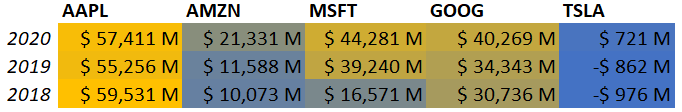
\includegraphics[scale=0.8]{heatmap.png}
        \caption{Net Profits for Apple, Amazon, Microsoft, Alphabet and Tesla }
\end{table}

\subsection{Interesting graph}
The following graph uses 5 colours that are generally easy to distinguish for colour-blind people. It shows cumulative returns over the 1-year period from November 23\textsuperscript{rd} 2020 to November 22\textsuperscript{nd} 2021 of the 5 biggest US companies by market capitalization.
 \begin{figure}[H]
   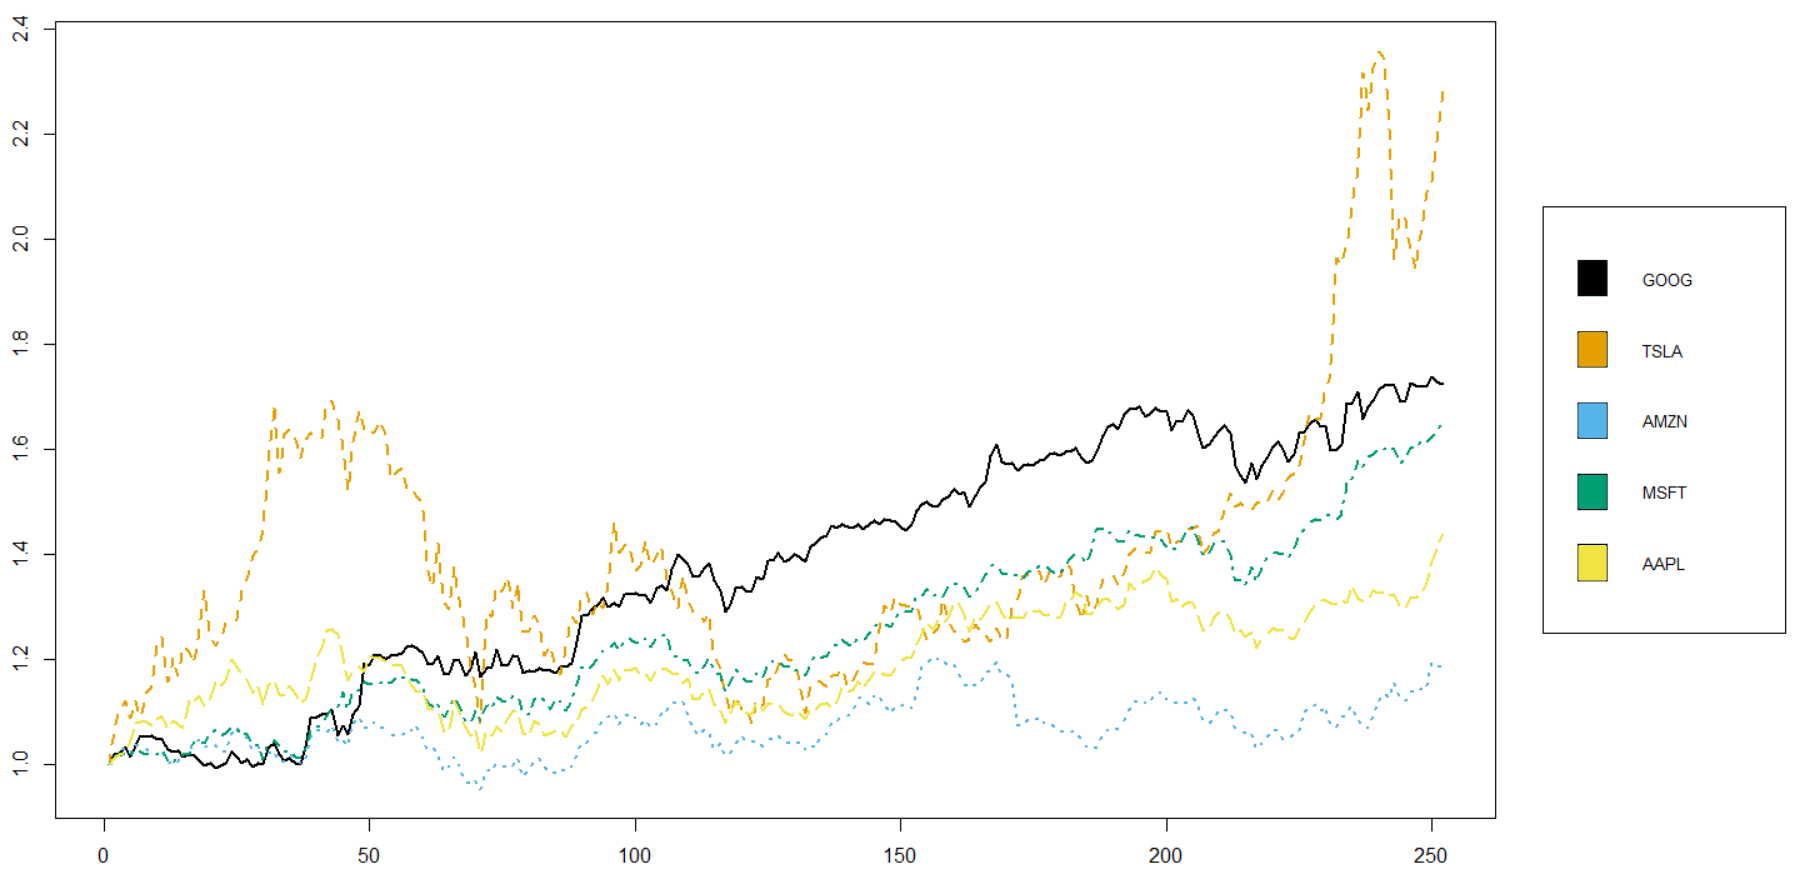
\includegraphics[scale=0.25]{cumreturns.png}
    \caption{Cumulative stock returns of the 5 biggest US companies, since Nov 23\textsuperscript{rd} 2020}
\end{figure}

\section{Conclusion}
Here we cite some more papers to show that we can comfortably work with .bib files. One example is \cite{Black1973}. Other possibly interesting readings are \cite{pursiainen2020cultural} and \cite{barras2020skill}, which were both recently published in the \textit{Journal of Finance}.

\newpage

\printbibliography

\end{document}